\documentclass[11pt,a4paper]{article}

% ── Packages ──
\usepackage[margin=2.5cm]{geometry}
\usepackage{amsmath,amssymb}
\usepackage{booktabs}
\usepackage{xcolor}
\usepackage{tikz}
\usepackage{pgfplots}
\pgfplotsset{compat=1.18}
\usetikzlibrary{
  arrows.meta,
  calc,
  positioning,
  shapes.geometric,
  fit,
  backgrounds,
  matrix
}
\usepackage{hyperref}
\usepackage{subcaption}
\usepackage{float}
\usepackage{array}
\usepackage{fancyhdr}
\usepackage{titlesec}

% ── Colors ──
\definecolor{dinoblue}{RGB}{41,98,168}
\definecolor{rgbgreen}{RGB}{34,139,34}
\definecolor{thermalred}{RGB}{178,34,34}
\definecolor{glasscol}{RGB}{52,152,219}
\definecolor{metalcol}{RGB}{149,165,166}
\definecolor{papercol}{RGB}{243,156,18}
\definecolor{plasticcol}{RGB}{46,204,113}
\definecolor{blockblue}{RGB}{220,235,252}
\definecolor{blockred}{RGB}{252,225,220}
\definecolor{blockgreen}{RGB}{220,252,225}
\definecolor{blockgray}{RGB}{240,240,240}
\definecolor{headblue}{RGB}{30,70,130}

% ── Page style ──
\pagestyle{fancy}
\fancyhf{}
\fancyhead[L]{\small\textcolor{gray}{DINOv2 Material Classification --- Executive Summary}}
\fancyhead[R]{\small\textcolor{gray}{\thepage}}
\renewcommand{\headrulewidth}{0.4pt}

% ── Title formatting ──
\titleformat{\section}{\Large\bfseries\color{headblue}}{\thesection}{1em}{}
\titleformat{\subsection}{\large\bfseries\color{headblue!80}}{\thesubsection}{1em}{}

% ── Macros ──
\newcommand{\cls}{\texttt{[CLS]}}

\begin{document}

% ══════════════════════════════════════════════════════════════
%  TITLE (no title page)
% ══════════════════════════════════════════════════════════════
\begin{center}
  {\LARGE\bfseries\color{headblue} Municipal Waste Classification}\\[0.3cm]
  {\LARGE\bfseries\color{headblue} with DINOv2 Embeddings}\\[0.5cm]
  {\large\color{gray} RGB and Thermal Pipeline Performance}\\[0.3cm]
  {\normalsize\today}
\end{center}

\vspace{0.5cm}

% ══════════════════════════════════════════════════════════════
%  1  OVERVIEW
% ══════════════════════════════════════════════════════════════
\section{Overview}

This report summarizes the performance of two single-modal classification pipelines for conveyor belt waste sorting into four material classes: \textbf{glass}, \textbf{metal}, \textbf{paper}, and \textbf{plastic}. Both pipelines use a frozen DINOv2 ViT-L/14 backbone (${\sim}$304M parameters) as a feature extractor, with only a lightweight attention pooling layer and MLP classification head trained (${\sim}$528K trainable parameters each, 0.17\% of backbone). All results are from \textbf{5-fold stratified cross-validation} on 550 labeled tracklets from 19 experiment videos.


% ══════════════════════════════════════════════════════════════
%  2  RGB PIPELINE
% ══════════════════════════════════════════════════════════════
\section{RGB Pipeline}

\subsection{Architecture}

\begin{figure}[H]
\centering
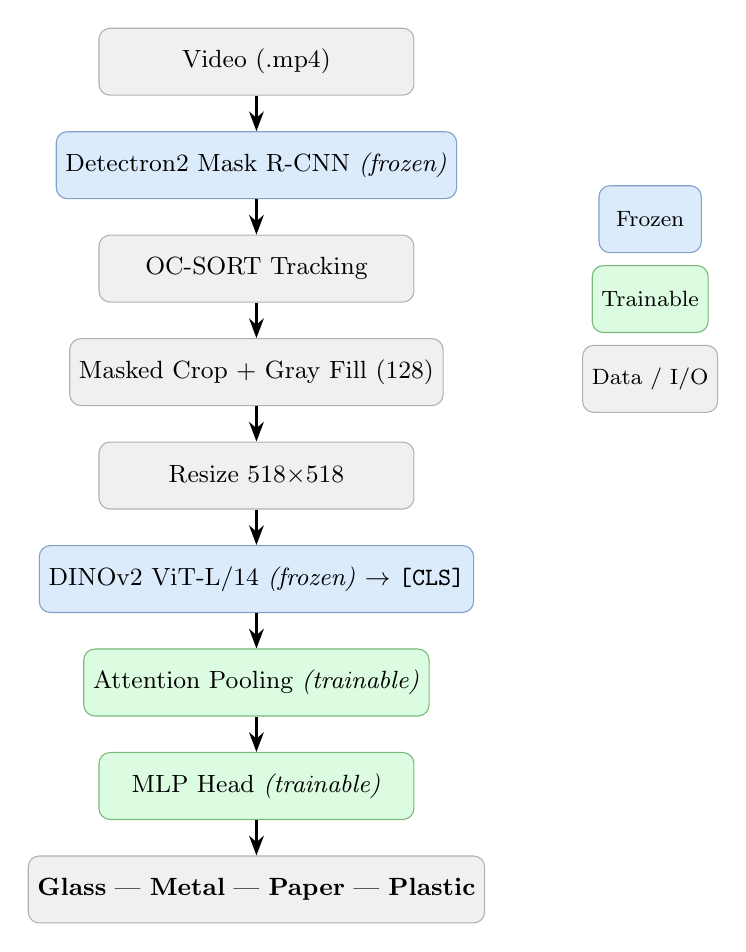
\begin{tikzpicture}[
  block/.style={draw, rounded corners=4pt, minimum height=0.85cm,
                minimum width=4cm, align=center, font=\small},
  frozen/.style={block, fill=blockblue, draw=dinoblue!60},
  train/.style={block, fill=blockgreen, draw=rgbgreen!60},
  data/.style={block, fill=blockgray, draw=black!30},
  arr/.style={-{Stealth[length=2.5mm]}, thick},
  node distance=0.45cm
]

\node[data] (video) {Video (.mp4)};
\node[frozen, below=of video] (det) {Detectron2 Mask R-CNN \textit{(frozen)}};
\node[data, below=of det] (track) {OC-SORT Tracking};
\node[data, below=of track] (mask) {Masked Crop + Gray Fill (128)};
\node[data, below=of mask] (resize) {Resize 518$\times$518};
\node[frozen, below=of resize] (dino) {DINOv2 ViT-L/14 \textit{(frozen)} $\to$ \cls{}};
\node[train, below=of dino] (pool) {Attention Pooling \textit{(trainable)}};
\node[train, below=of pool] (head) {MLP Head \textit{(trainable)}};
\node[data, below=of head] (out) {\textbf{Glass} | \textbf{Metal} | \textbf{Paper} | \textbf{Plastic}};

\draw[arr] (video) -- (det);
\draw[arr] (det) -- (track);
\draw[arr] (track) -- (mask);
\draw[arr] (mask) -- (resize);
\draw[arr] (resize) -- (dino);
\draw[arr] (dino) -- (pool);
\draw[arr] (pool) -- (head);
\draw[arr] (head) -- (out);

% Legend
\node[frozen, minimum width=1.3cm, font=\footnotesize] at (5, -2) (leg1) {Frozen};
\node[train, minimum width=1.3cm, font=\footnotesize, below=0.15cm of leg1] (leg2) {Trainable};
\node[data, minimum width=1.3cm, font=\footnotesize, below=0.15cm of leg2] (leg3) {Data / I/O};

\end{tikzpicture}
\caption{RGB classification pipeline. Detection and DINOv2 are frozen; only the attention pool and MLP head are trained (${\sim}$528K parameters).}
\label{fig:rgb_pipeline}
\end{figure}

\subsection{Overall Results}

\begin{table}[H]
\centering
\caption{RGB pipeline: 5-fold stratified CV results (550 tracklets, 19 videos).}
\label{tab:rgb_overall}
\begin{tabular}{@{}lc@{}}
\toprule
\textbf{Metric} & \textbf{Value} \\
\midrule
Mean Accuracy & $0.9509 \pm 0.0093$ \\
Mean Macro F1 & $0.9507 \pm 0.0110$ \\
Pooled Accuracy & $0.9509$ \\
Pooled Macro F1 & $0.9508$ \\
Total Errors & 27 / 550 \\
\bottomrule
\end{tabular}
\end{table}

\subsection{Per-Class Metrics}

\begin{table}[H]
\centering
\caption{RGB per-class metrics (pooled across all 5 folds).}
\label{tab:rgb_perclass}
\begin{tabular}{@{}lcccc@{}}
\toprule
\textbf{Class} & \textbf{Precision} & \textbf{Recall} & \textbf{F1} & \textbf{Count} \\
\midrule
Glass   & 0.9776 & 0.9924 & 0.9850 & 132 \\
Metal   & 0.9209 & 0.9771 & 0.9481 & 131 \\
Paper   & 0.9570 & 0.9082 & 0.9319 & 98 \\
Plastic & 0.9511 & 0.9259 & 0.9383 & 189 \\
\bottomrule
\end{tabular}
\end{table}

\subsection{Confusion Matrix}

\begin{figure}[H]
\centering
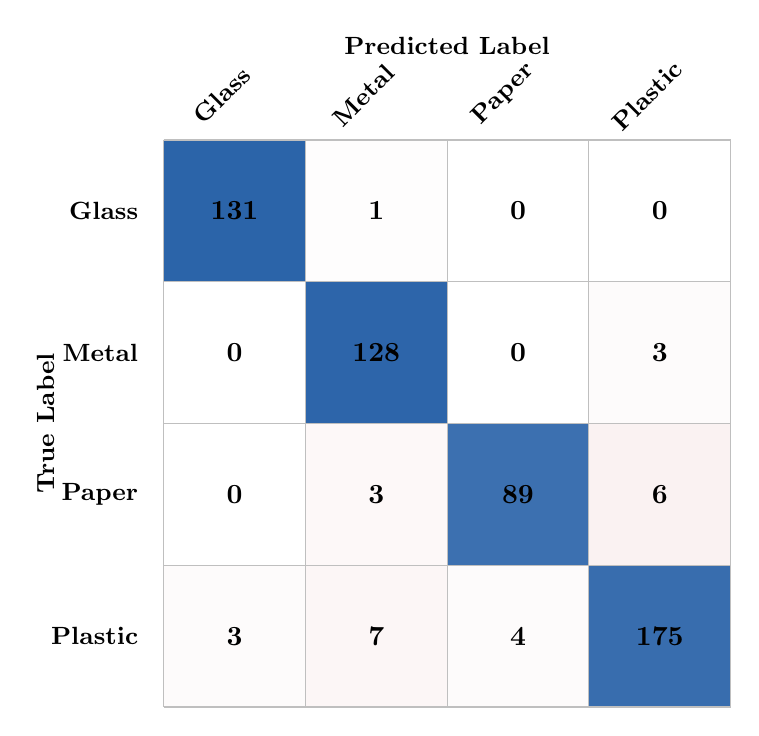
\begin{tikzpicture}[font=\small]
  % Row 0: Glass  (131, 1, 0, 0)  total=132
  \fill[dinoblue!99!white] (0, 0) rectangle (1.8, 1.8);
  \fill[thermalred!1!white] (1.8, 0) rectangle (3.6, 1.8);
  \fill[white] (3.6, 0) rectangle (5.4, 1.8);
  \fill[white] (5.4, 0) rectangle (7.2, 1.8);
  % Row 1: Metal  (0, 128, 0, 3)  total=131
  \fill[white] (0, -1.8) rectangle (1.8, 0);
  \fill[dinoblue!98!white] (1.8, -1.8) rectangle (3.6, 0);
  \fill[white] (3.6, -1.8) rectangle (5.4, 0);
  \fill[thermalred!2!white] (5.4, -1.8) rectangle (7.2, 0);
  % Row 2: Paper  (0, 3, 89, 6)  total=98
  \fill[white] (0, -3.6) rectangle (1.8, -1.8);
  \fill[thermalred!3!white] (1.8, -3.6) rectangle (3.6, -1.8);
  \fill[dinoblue!91!white] (3.6, -3.6) rectangle (5.4, -1.8);
  \fill[thermalred!6!white] (5.4, -3.6) rectangle (7.2, -1.8);
  % Row 3: Plastic  (3, 7, 4, 175)  total=189
  \fill[thermalred!2!white] (0, -5.4) rectangle (1.8, -3.6);
  \fill[thermalred!4!white] (1.8, -5.4) rectangle (3.6, -3.6);
  \fill[thermalred!2!white] (3.6, -5.4) rectangle (5.4, -3.6);
  \fill[dinoblue!93!white] (5.4, -5.4) rectangle (7.2, -3.6);

  % Grid lines
  \foreach \i in {0,...,4} {
    \draw[gray!50] (\i*1.8, 1.8) -- (\i*1.8, -5.4);
    \draw[gray!50] (0, 1.8-\i*1.8) -- (7.2, 1.8-\i*1.8);
  }

  % Values
  \node[font=\normalsize\bfseries] at (0.9, 0.9) {131};
  \node[font=\normalsize\bfseries] at (2.7, 0.9) {1};
  \node[font=\normalsize\bfseries] at (4.5, 0.9) {0};
  \node[font=\normalsize\bfseries] at (6.3, 0.9) {0};

  \node[font=\normalsize\bfseries] at (0.9, -0.9) {0};
  \node[font=\normalsize\bfseries] at (2.7, -0.9) {128};
  \node[font=\normalsize\bfseries] at (4.5, -0.9) {0};
  \node[font=\normalsize\bfseries] at (6.3, -0.9) {3};

  \node[font=\normalsize\bfseries] at (0.9, -2.7) {0};
  \node[font=\normalsize\bfseries] at (2.7, -2.7) {3};
  \node[font=\normalsize\bfseries] at (4.5, -2.7) {89};
  \node[font=\normalsize\bfseries] at (6.3, -2.7) {6};

  \node[font=\normalsize\bfseries] at (0.9, -4.5) {3};
  \node[font=\normalsize\bfseries] at (2.7, -4.5) {7};
  \node[font=\normalsize\bfseries] at (4.5, -4.5) {4};
  \node[font=\normalsize\bfseries] at (6.3, -4.5) {175};

  % Column labels (predicted)
  \node[font=\small\bfseries, rotate=45, anchor=south] at (0.9, 2.2) {Glass};
  \node[font=\small\bfseries, rotate=45, anchor=south] at (2.7, 2.2) {Metal};
  \node[font=\small\bfseries, rotate=45, anchor=south] at (4.5, 2.2) {Paper};
  \node[font=\small\bfseries, rotate=45, anchor=south] at (6.3, 2.2) {Plastic};

  % Row labels (true)
  \node[font=\small\bfseries, anchor=east] at (-0.2, 0.9) {Glass};
  \node[font=\small\bfseries, anchor=east] at (-0.2, -0.9) {Metal};
  \node[font=\small\bfseries, anchor=east] at (-0.2, -2.7) {Paper};
  \node[font=\small\bfseries, anchor=east] at (-0.2, -4.5) {Plastic};

  \node[font=\small\bfseries, rotate=90] at (-1.5, -1.8) {True Label};
  \node[font=\small\bfseries] at (3.6, 3.0) {Predicted Label};
\end{tikzpicture}
\caption{RGB confusion matrix (pooled across 5 folds). Only 27 misclassifications out of 550. Glass is near-perfect (131/132). Most confusion: plastic$\leftrightarrow$metal (10) and paper$\leftrightarrow$plastic (10).}
\label{fig:rgb_confusion}
\end{figure}


% ══════════════════════════════════════════════════════════════
%  3  THERMAL PIPELINE
% ══════════════════════════════════════════════════════════════
\section{Thermal Pipeline}

\subsection{Architecture}

\begin{figure}[H]
\centering
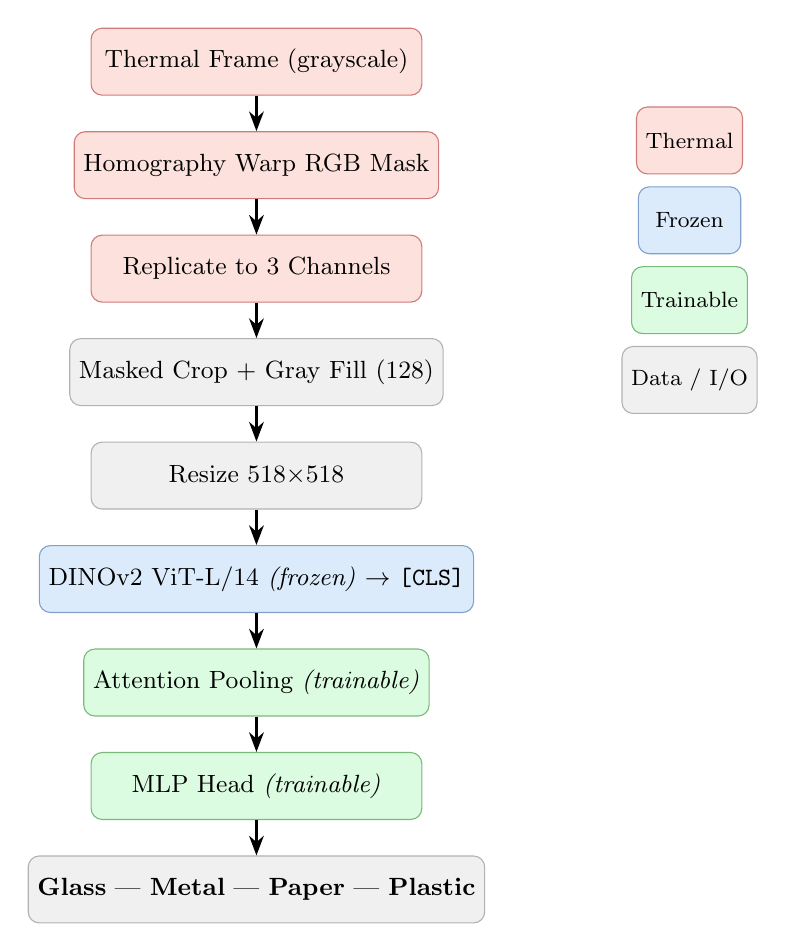
\begin{tikzpicture}[
  block/.style={draw, rounded corners=4pt, minimum height=0.85cm,
                minimum width=4.2cm, align=center, font=\small},
  frozen/.style={block, fill=blockblue, draw=dinoblue!60},
  train/.style={block, fill=blockgreen, draw=rgbgreen!60},
  data/.style={block, fill=blockgray, draw=black!30},
  thermal/.style={block, fill=blockred, draw=thermalred!60},
  arr/.style={-{Stealth[length=2.5mm]}, thick},
  node distance=0.45cm
]

\node[thermal] (frame) {Thermal Frame (grayscale)};
\node[thermal, below=of frame] (warp) {Homography Warp RGB Mask};
\node[thermal, below=of warp] (rep) {Replicate to 3 Channels};
\node[data, below=of rep] (mask) {Masked Crop + Gray Fill (128)};
\node[data, below=of mask] (resize) {Resize 518$\times$518};
\node[frozen, below=of resize] (dino) {DINOv2 ViT-L/14 \textit{(frozen)} $\to$ \cls{}};
\node[train, below=of dino] (pool) {Attention Pooling \textit{(trainable)}};
\node[train, below=of pool] (head) {MLP Head \textit{(trainable)}};
\node[data, below=of head] (out) {\textbf{Glass} | \textbf{Metal} | \textbf{Paper} | \textbf{Plastic}};

\draw[arr] (frame) -- (warp);
\draw[arr] (warp) -- (rep);
\draw[arr] (rep) -- (mask);
\draw[arr] (mask) -- (resize);
\draw[arr] (resize) -- (dino);
\draw[arr] (dino) -- (pool);
\draw[arr] (pool) -- (head);
\draw[arr] (head) -- (out);

% Legend
\node[thermal, minimum width=1.3cm, font=\footnotesize] at (5.5, -1) (leg0) {Thermal};
\node[frozen, minimum width=1.3cm, font=\footnotesize, below=0.15cm of leg0] (leg1) {Frozen};
\node[train, minimum width=1.3cm, font=\footnotesize, below=0.15cm of leg1] (leg2) {Trainable};
\node[data, minimum width=1.3cm, font=\footnotesize, below=0.15cm of leg2] (leg3) {Data / I/O};

\end{tikzpicture}
\caption{Thermal classification pipeline. Thermal-specific steps (red) include homography-based mask warping from RGB space and grayscale-to-3-channel replication for DINOv2 compatibility.}
\label{fig:thermal_pipeline}
\end{figure}

\subsection{Overall Results}

\begin{table}[H]
\centering
\caption{Thermal pipeline: 5-fold stratified CV results (550 tracklets, 19 videos).}
\label{tab:thermal_overall}
\begin{tabular}{@{}lc@{}}
\toprule
\textbf{Metric} & \textbf{Value} \\
\midrule
Mean Accuracy & $0.9127 \pm 0.0384$ \\
Mean Macro F1 & $0.9056 \pm 0.0405$ \\
Pooled Accuracy & $0.9127$ \\
Pooled Macro F1 & $0.9055$ \\
Total Errors & 48 / 550 \\
\bottomrule
\end{tabular}
\end{table}

\subsection{Per-Class Metrics}

\begin{table}[H]
\centering
\caption{Thermal per-class metrics (pooled across all 5 folds).}
\label{tab:thermal_perclass}
\begin{tabular}{@{}lcccc@{}}
\toprule
\textbf{Class} & \textbf{Precision} & \textbf{Recall} & \textbf{F1} & \textbf{Count} \\
\midrule
Glass   & 0.9559 & 0.9848 & 0.9701 & 132 \\
Metal   & 0.9380 & 0.9237 & 0.9308 & 131 \\
Paper   & 0.7921 & 0.8163 & 0.8040 & 98 \\
Plastic & 0.9293 & 0.9048 & 0.9169 & 189 \\
\bottomrule
\end{tabular}
\end{table}

\subsection{Confusion Matrix}

\begin{figure}[H]
\centering
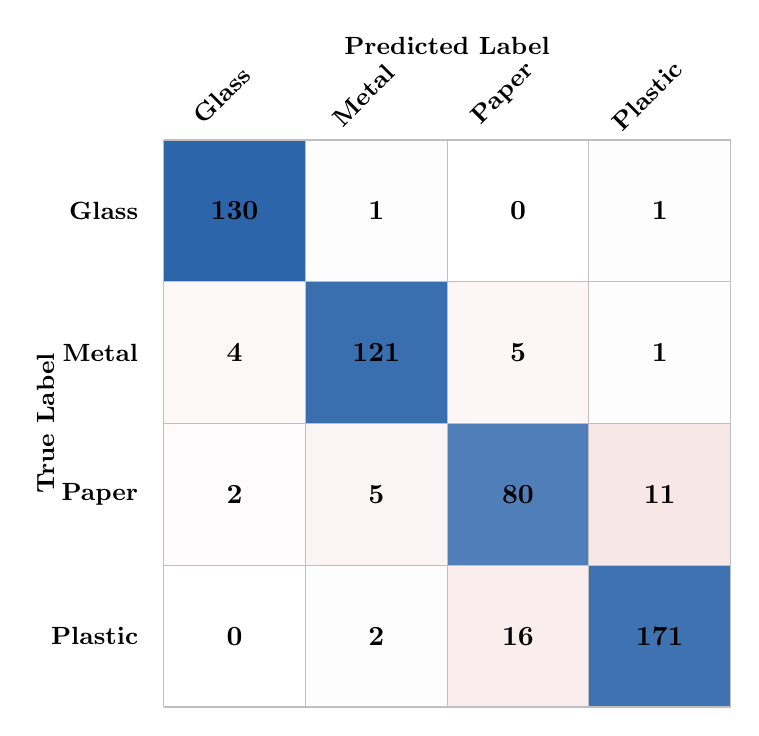
\begin{tikzpicture}[font=\small]
  % Row 0: Glass  (130, 1, 0, 1)  total=132
  \fill[dinoblue!98!white] (0, 0) rectangle (1.8, 1.8);
  \fill[thermalred!1!white] (1.8, 0) rectangle (3.6, 1.8);
  \fill[white] (3.6, 0) rectangle (5.4, 1.8);
  \fill[thermalred!1!white] (5.4, 0) rectangle (7.2, 1.8);
  % Row 1: Metal  (4, 121, 5, 1)  total=131
  \fill[thermalred!3!white] (0, -1.8) rectangle (1.8, 0);
  \fill[dinoblue!92!white] (1.8, -1.8) rectangle (3.6, 0);
  \fill[thermalred!4!white] (3.6, -1.8) rectangle (5.4, 0);
  \fill[thermalred!1!white] (5.4, -1.8) rectangle (7.2, 0);
  % Row 2: Paper  (2, 5, 80, 11)  total=98
  \fill[thermalred!2!white] (0, -3.6) rectangle (1.8, -1.8);
  \fill[thermalred!5!white] (1.8, -3.6) rectangle (3.6, -1.8);
  \fill[dinoblue!82!white] (3.6, -3.6) rectangle (5.4, -1.8);
  \fill[thermalred!11!white] (5.4, -3.6) rectangle (7.2, -1.8);
  % Row 3: Plastic  (0, 2, 16, 171)  total=189
  \fill[white] (0, -5.4) rectangle (1.8, -3.6);
  \fill[thermalred!1!white] (1.8, -5.4) rectangle (3.6, -3.6);
  \fill[thermalred!8!white] (3.6, -5.4) rectangle (5.4, -3.6);
  \fill[dinoblue!90!white] (5.4, -5.4) rectangle (7.2, -3.6);

  % Grid lines
  \foreach \i in {0,...,4} {
    \draw[gray!50] (\i*1.8, 1.8) -- (\i*1.8, -5.4);
    \draw[gray!50] (0, 1.8-\i*1.8) -- (7.2, 1.8-\i*1.8);
  }

  % Values
  \node[font=\normalsize\bfseries] at (0.9, 0.9) {130};
  \node[font=\normalsize\bfseries] at (2.7, 0.9) {1};
  \node[font=\normalsize\bfseries] at (4.5, 0.9) {0};
  \node[font=\normalsize\bfseries] at (6.3, 0.9) {1};

  \node[font=\normalsize\bfseries] at (0.9, -0.9) {4};
  \node[font=\normalsize\bfseries] at (2.7, -0.9) {121};
  \node[font=\normalsize\bfseries] at (4.5, -0.9) {5};
  \node[font=\normalsize\bfseries] at (6.3, -0.9) {1};

  \node[font=\normalsize\bfseries] at (0.9, -2.7) {2};
  \node[font=\normalsize\bfseries] at (2.7, -2.7) {5};
  \node[font=\normalsize\bfseries] at (4.5, -2.7) {80};
  \node[font=\normalsize\bfseries] at (6.3, -2.7) {11};

  \node[font=\normalsize\bfseries] at (0.9, -4.5) {0};
  \node[font=\normalsize\bfseries] at (2.7, -4.5) {2};
  \node[font=\normalsize\bfseries] at (4.5, -4.5) {16};
  \node[font=\normalsize\bfseries] at (6.3, -4.5) {171};

  % Column labels (predicted)
  \node[font=\small\bfseries, rotate=45, anchor=south] at (0.9, 2.2) {Glass};
  \node[font=\small\bfseries, rotate=45, anchor=south] at (2.7, 2.2) {Metal};
  \node[font=\small\bfseries, rotate=45, anchor=south] at (4.5, 2.2) {Paper};
  \node[font=\small\bfseries, rotate=45, anchor=south] at (6.3, 2.2) {Plastic};

  % Row labels (true)
  \node[font=\small\bfseries, anchor=east] at (-0.2, 0.9) {Glass};
  \node[font=\small\bfseries, anchor=east] at (-0.2, -0.9) {Metal};
  \node[font=\small\bfseries, anchor=east] at (-0.2, -2.7) {Paper};
  \node[font=\small\bfseries, anchor=east] at (-0.2, -4.5) {Plastic};

  \node[font=\small\bfseries, rotate=90] at (-1.5, -1.8) {True Label};
  \node[font=\small\bfseries] at (3.6, 3.0) {Predicted Label};
\end{tikzpicture}
\caption{Thermal confusion matrix (pooled across 5 folds). 48 misclassifications. Paper$\leftrightarrow$plastic confusion dominates (27 errors), reflecting similar thermal signatures for these materials.}
\label{fig:thermal_confusion}
\end{figure}


% ══════════════════════════════════════════════════════════════
%  4  COMPARATIVE SUMMARY
% ══════════════════════════════════════════════════════════════
\section{Comparative Summary}

\begin{figure}[H]
\centering
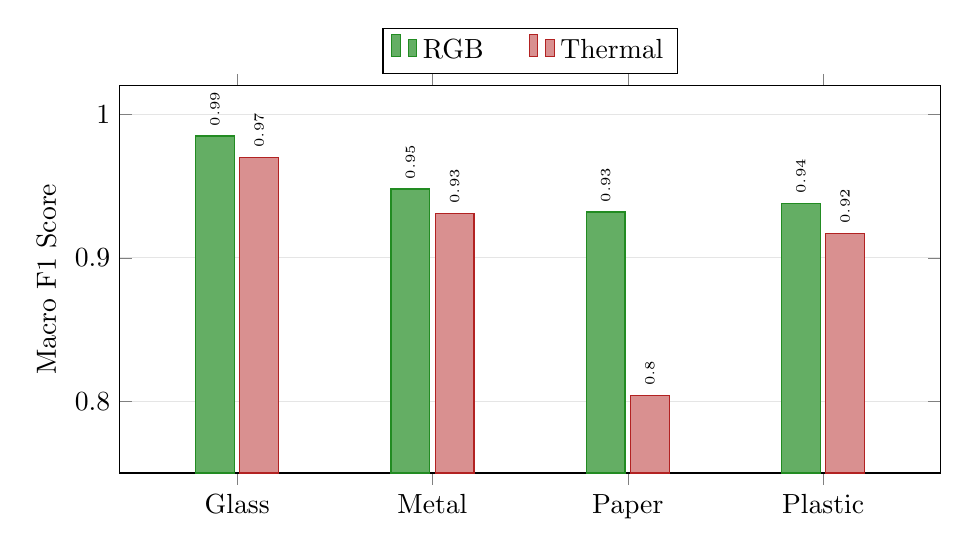
\begin{tikzpicture}
\begin{axis}[
  ybar,
  bar width=14pt,
  width=12cm,
  height=6.5cm,
  ylabel={Macro F1 Score},
  symbolic x coords={Glass, Metal, Paper, Plastic},
  xtick=data,
  ymin=0.75, ymax=1.02,
  ymajorgrids=true,
  grid style={gray!20},
  legend style={
    at={(0.5, 1.15)},
    anchor=north,
    legend columns=2,
    /tikz/every even column/.append style={column sep=0.5cm}
  },
  nodes near coords,
  every node near coord/.append style={font=\tiny, rotate=90, anchor=west},
  enlarge x limits=0.2,
]
\addplot[fill=rgbgreen!70, draw=rgbgreen] coordinates {
  (Glass, 0.985) (Metal, 0.948) (Paper, 0.932) (Plastic, 0.938)
};
\addplot[fill=thermalred!50, draw=thermalred] coordinates {
  (Glass, 0.970) (Metal, 0.931) (Paper, 0.804) (Plastic, 0.917)
};
\legend{RGB, Thermal}
\end{axis}
\end{tikzpicture}
\caption{Per-class F1 comparison: RGB vs.\ Thermal. RGB outperforms thermal on all classes, with the largest gap on paper (0.932 vs.\ 0.804).}
\label{fig:comparison_chart}
\end{figure}

\noindent\textbf{Key takeaways:}
RGB outperforms thermal overall (\textbf{95.1\%} vs.\ \textbf{90.6\%} macro F1), with both modalities achieving strong results using the same frozen DINOv2 backbone and identical trainable architecture. Glass is near-perfect in both pipelines (F1 $\geq$ 0.97). Paper is the hardest class for both modalities, but especially for thermal (F1 = 0.804 vs.\ 0.932), reflecting inherently similar thermal signatures between paper and plastic. The thermal pipeline also exhibits higher variance across folds ($\pm$0.04 vs.\ $\pm$0.01), suggesting that thermal features are more sensitive to the specific train/test partition. Despite lower standalone accuracy, the thermal modality captures complementary material properties (thermal conductivity, emissivity) that can benefit a fusion approach.

\end{document}
